

The idea of using a single-electron density to approximate the intricate many-body interactions in multielectronic systems continues to be an attractive pursuit to develop better and computationally cheap functionals, in order to facilitate our understanding on the fundamental properties of materials thus driving the discovery of novel materials that do not exist in the current material space. It is therefore not surprising that a `zoo'\cite{goerigk2019trip} of more than 200 density functionals\cite{mardirossian2017thirty} have been developed to date, making it a profound challenge for DFT practitioners to choose the most appropriate functional to be applied for a specific modelling problem at hand, if not simply resolving to the most popular one(s).\cite{kruse2012standard}

In this regard, benchmarking the performance of DFAs in reproducing the reference material property data, derived either experimentally or from high-level theoretical calculations (such as coupled-cluster theory\cite{bartlett2007coupled}) becomes a critical component in the research community of DFT. There are a few key rationales behind the efforts in carefully collating and assembling comprehensive benchmark sets: (1) Each DFA was designed and developed under some specific assumptions and approximations to the multielectronic behaviours in real materials, a quantitative measure is needed in order for us to assess how good these approximations are. (2) It is no surprise that electrons behave differently in different material systems, such as metals and insulators. Therefore, it is important to calibrate DFAs that are designed to satisfy different `boundary conditions' on their capabilities in correctly predicting the behaviours of different materials.  On this regard, whilst the construction of a universal DFA may be a desirable pursuit, there is no compelling reason to believe such a functional, if it exists, would be easy to implement or numerically efficient.\cite{DFT_exchange} (3) By understanding the limitations in different functionals, for example, GGA being able to produce reliable structures for solids but failed for estimating the band gap energies [\cref{fig:DFT_bandgap} (c,d)], it can guide the future designs and choices of DFAs for future improvements in electronic structure theory and better results in materials modelling. This is particularly useful when we can quantify the uncertainties in reproducing the benchmark values with a specific DFA. Finally, (4) it helps establishing practical standards for the computational chemistry and materials science community, which encourages data sharing, as well as increases the trust and transferability of computational modelling as an essential tool for scientific discoveries.\cite{DFT_exchange}


\begin{figure}[tb]
    \centering
    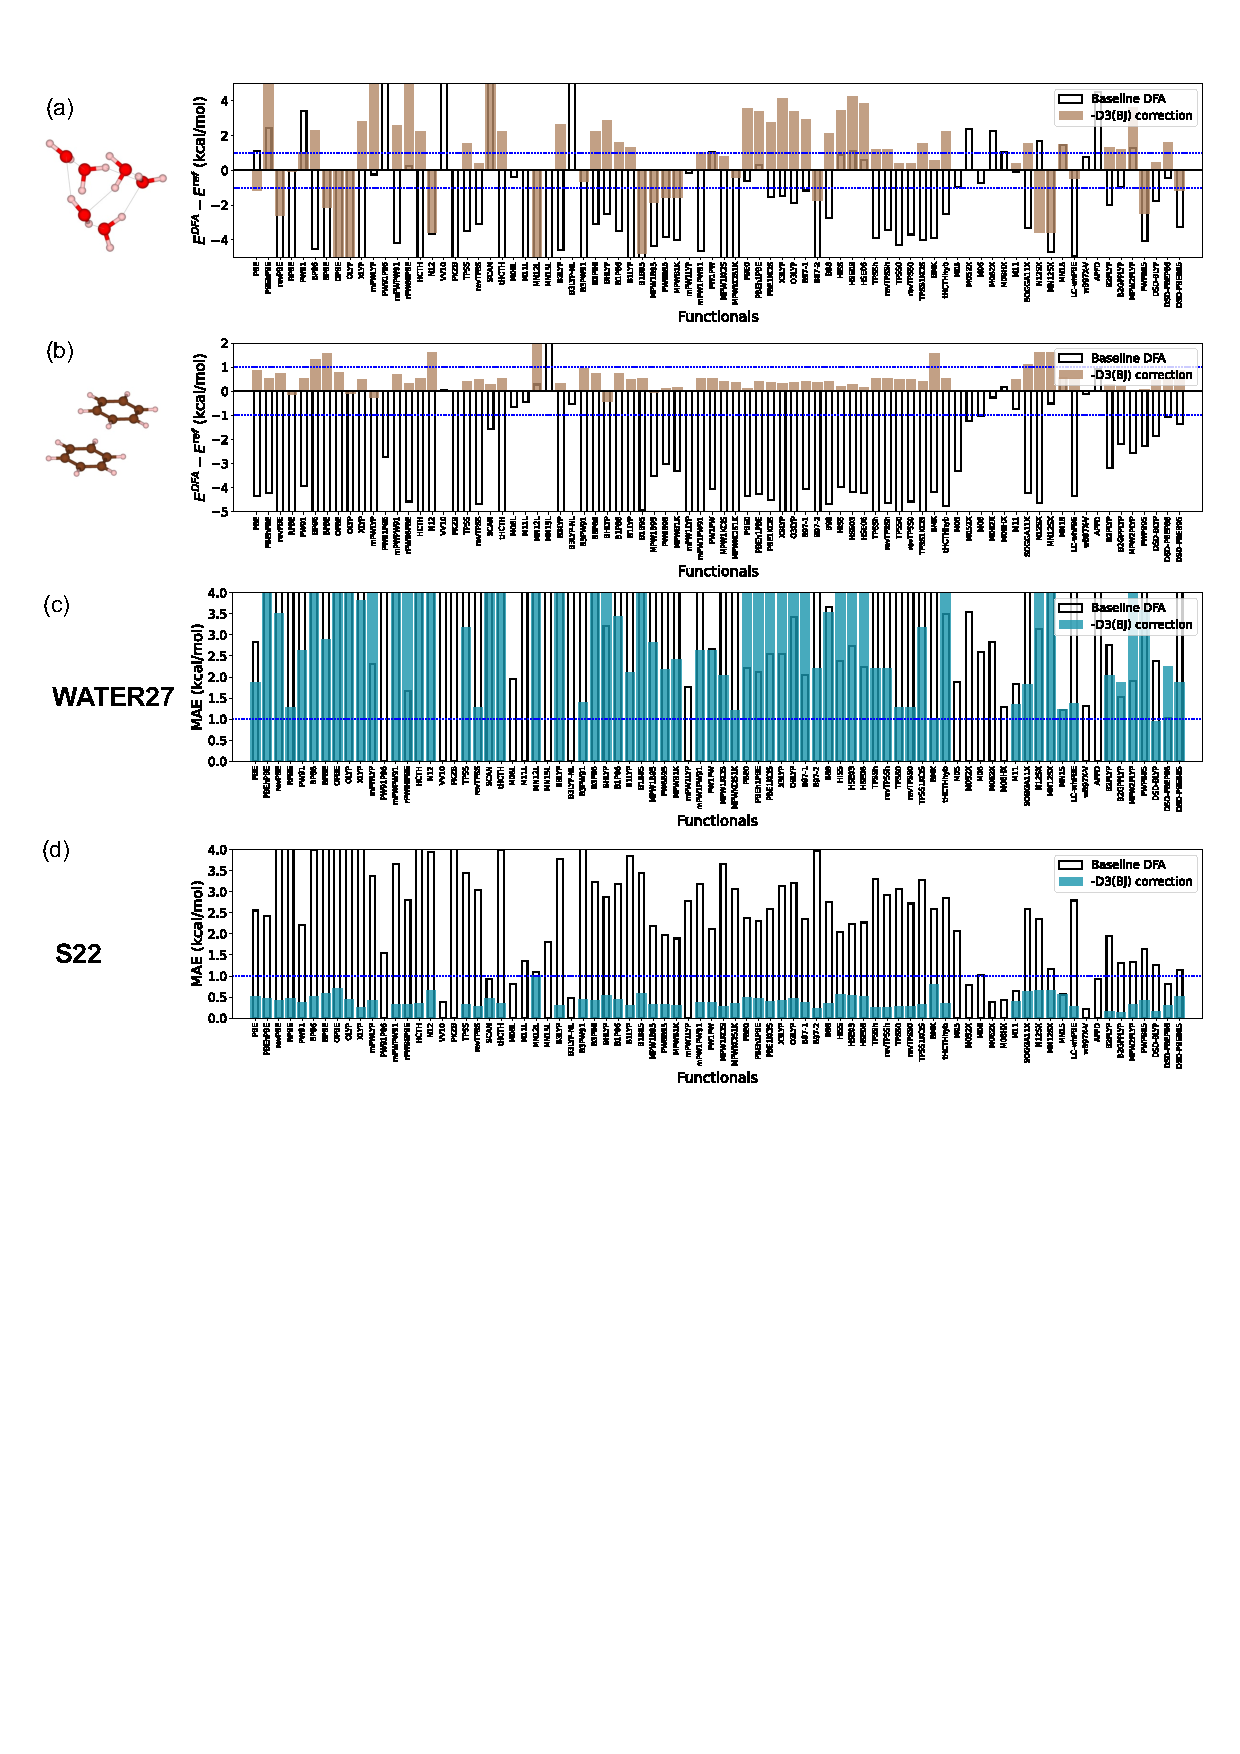
\includegraphics[width=\textwidth]{DFA_benchmarks.pdf}
    \caption{Benchmarking the performances of DFAs for determining the energetic stabilities  of model chemical systems for the purposes of assessing their applicability. (a) Binding energy of a small hydrogen bonded (\ce{H2O})$_6$ cluster as in the WATER27 (binding energies for small neutral, protonated and deprotonated water clusters) benchmark set,\cite{bryantsev2009evaluation} where the reference value $E^{ref}$ was reported in \citet{manna2017conventional} at the MP2/CBS+$\Delta$CCSD(T) level of theory. (b) Binding energy of a dispersion force bounded benzene dimer from the S22 (noncovalent interaction energies for 22 dimers of small molecules) benchmark set,\cite{jurevcka2006benchmark} with the reference value determined at the CCSD(T)/CBS level that is subsequently corrected with $\delta_{\mbox{\scriptsize{MP2}}}^{\mbox{\scriptsize{CCSD(T)}}}$ values.\cite{marshall2011basis} In (a-b), the performances of DFAs are measured based on the unsigned difference between the energies determined by a given DFA and the reference value, namely $\Delta E=E^{DFA}-E^{ref}$, which provides an indication on whether a specific DFA tends to under- or over-bind the molecular complex. The mean absolute errors (MAE) for DFAs in determining the binding energies of molecular complexes, which are determined as $\frac{1}{N}\sum_{i=1}^{N}|\Delta E_i|$ across all $N$ molecules in the WATER27 (c) and S22 (d) sets for each DFA examined. In all figures, the performance of the baseline DFAs (empty bars), and those that are dispersion-interaction-corrected (filled bars, if available) by Grimme's D3(BJ) scheme.\cite{grimme2010consistent,grimme2011effect} The blue dashed lines designate the position where $|\Delta E|$ or MAE is  1 kcal/mol, the limit within with the DFAs are considered as being able to predict the molecular binding energies with the so-called `chemical accuracy'. All data presented here are extracted from the new GMTKN55 quantum chemistry benchmark database.\cite{goerigk2017look}}
    \label{fig:DFA_benchmarks}
\end{figure}


Here, we shall provide   high-level overviews on the key features in some of the well-known benchmark sets in the community. 

In the chemistry community, the GMTKN55\cite{goerigk2017look} (\textbf{G}eneral \textbf{M}ain group \textbf{T}hermochemistry \textbf{K}inetic \textbf{N}on-covalent interactions) database, which is an extended version to its popular predecessor GMTKN30,\cite{goerigk2011efficient} represents one of the most comprehensive benchmark for main group chemistries. It tested the performance of 217 dispersion-corrected and -uncorrected DFAs in reproducing 1505 reference values of relative energies that were primarily determined from high-level wavefunction theory calculations. It is the \emph{relative energy}  because every system that has been benchmarked can be casted into the form of reactants$\to$products, with $\Delta E=E_{total}(\mbox{products})-E_{total}(\mbox{reactants})$. 

In a high-level overview, the GMTKN database is organised in such a way that the performances of individual DFA, measured in terms of the deviation of DFA-determined relative energies to the corresponding reference values, can be assessed on the levels of (1) A specific chemical system. For instance, \cref{fig:DFA_benchmarks}(a) and (b) show the relative unsigned errors in calculating the interaction energies of a small hydrogen-bonded water cluster and a $\pi$-stacked benzene dimers. It  can be seen that for purely dispersion-bounded benzene dimers, the inclusion of -D3(BJ) corrections consistently improves the results in determining the interaction energy, but less so for water clusters that are strongly bounded by dipole-dipole interactions. (2) A set of chemically similar systems, such as the WATER27 and S22 sets shown in \cref{fig:DFA_benchmarks}(c) and (d) whereby the molecular systems within a given set share some commonalities in the electronic natures that determine their interaction strengths, and thus the benchmark data reflects the capabilities of different functional designs in capturing those critical electronic behaviours in the systems. (3) Overall performances of DFAs (particularly within given rung of the Jacob's ladder) across the whole benchmark, providing an evidence-based and data-driven recommendation for the best DFAs across each rung of the Jacob's ladder, which, can often be used as a starting point for new research project. For example, in the context of high-throughput screening where high computational speed is required, GGA functional revPBE-D3\cite{zhang1998comment} would be the best choice, however, double-hybrid functionals are critical for accurate thermochemistry and non-covalent interactions. 

Of course, the use of double-hybrid functionals may not be always computationally feasible. In this case, a careful sift through the benchmark for alternatives lower-rung DFAs would be needed, which can be a costly exercise.  In this regard, \citet{gould2018diet} has put forward an interesting genetic-algorithm approach to construct a `diet-GMTKN55' benchmark consisting of only 100 representative chemical systems that are capable of closely reproducing error metrics from the full set. 

The capability for us to theoretically collate accurate reference data for molecular systems with wavefunction method can be largely attributed to the efficiency of localised basis functions in quantum chemistry calculations. This is in stark contrast to periodic solids, for which the use of planewave basis sets are the practical norm, making it become very expensive for post-Hartree-Fock correlation calculations. On the other hands, systems such as Mott insulators\cite{imada1998metal} and transition metal oxides\cite{tokura2003correlated} that exhibit strong electron correlation effects would require more specialised theoretical treatments\cite{georges2004strongly,imada2010electronic} that are beyond the scope of the present review. In this regard, most benchmark studies for solids would focus on comparing the DFT-derived properties with known experimental results [\cref{fig:DFT_bandgap}]. Here, we shall briefly outline a few exemplary studies/datasets that have been widely referred to in the past decade.

In solid-state DFT calculations, the choice of pseudopotential and the corresponding cutoff radius for each element plays a crucial role in balancing the computational accuracy and speed. For this, \citet{prandini2018precision} have compiled a benchmark of standard solid-state pseudopotential (SSSP). Through careful testing of the convergence behaviours in phonon frequencies, band structure, cohesive energy and pressure calculations, for each element in the periodic table, the authors have provided the optimum choice of pesudopotential type and the corresponding cut-off radius based on two criteria: SSSP-efficiency tailored for high-throughput materials screenings and SSSP-accuracy for high-accurate (\emph{e.g.} phonon) calculations. Different research groups often select different DFT codes as their default choice, in this regard, \citet{lejaeghere2016reproducibility} had compared the reproducibility of DFT calculations from 15 different solid-state DFT codes in 2016. Even though there is a lack of reference DFT implementation, the study has already found that, the continuous improvement in the software developments, the results obtained from mainstream DFT codes are essentially identical, only varying subtly due to differences in the numerical implementation. 

Molecular crystals represent a unique set of material systems which, on one hand, their long-ranged electronic structures need to be accounted for with periodic DFT, on the other hand, the atom-atom pairwise non-covalent interactions that plays an important role in holding the molecules together in their crystalline form, rely heavily on our knowledge in the development of dispersion-corrected DFT from quantum chemistry. With this, the X23 benchmark for molecular crystals\cite{otero2012benchmark,reilly2013understanding,dolgonos2019revised} has tabulated reference lattice constants and sublimation enthalpies for 23 crystals of small molecules, which are  corrected for thermal vibration and expansion effects from the corresponding experimental values. Benchmarking studies showed that dispersion-correction in DFT, which takes into account the many-body effect, tends to perform best in reproducing the lattice energies. It has also played a critical role in assessing the accuracy of atom-atom forcefields for fast, high-throughput organic crystal structure predictions,\cite{nyman2016accurate}  and validates the application of dispersion-corrected DFT as a useful post-prediction method for correcting the forcefield-derived lattice energies to provide better energetic ranking of the polymorph stabilities from structure predictions, which are reflected in the last two blind tests.\cite{reilly2016report,Hunnisett:aw5094}

Finally, in the past decade, we have seen the establishment and continuous evolution of large-scale high-throughput computational material databases, as represented by the Materials Project Database,\cite{jain_apl_mater} AFLOW Database,\cite{CURTAROLO2012218} Open Quantum Materials Database (OQMD),\cite{kirklin2015open} and 2D Materials Database.\cite{haastrup2018,gjerding2021recent} These databases, being assembled for $\sim$150 K up to $\sim 2$ M inorganic materials, contain results from DFT calculations with the underlying method carefully tested to ensure the results are sufficiently accurate and consistent throughout the database, have provided the community a set of benchmarks for standardising and sanity checking future DFT calculations, which has already significantly enhance our capabilities to cross-compare results from different literatures and discover new phenomena in functional materials based on existing knowledges.